%% Files that are needed for LaTeX processing (style + inputs) are available
%% relative to the download place in the directory ../inputs, the images in
%% ../img

\documentclass[compress]{beamer}

\usepackage[utf8]{inputenc}
\mode<presentation>{
   \usetheme{Boadilla}
   \hypersetup{pdfpagemode=FullScreen}
}
\setbeamertemplate{navigation symbols}{}

\usepackage{debian-links}

\title{Activity of communication}


\author{Sukhbir Singh, Andreas Tille}

%\institute{\Debian}
\institute{\link{http://www.debconf.org/debconf8/}{Debian Conference 8}}

\date{Banja Luka, July ??, 2011}

\begin{document}

\begin{frame}
  \titlepage
\end{frame}

\begin{frame}
  \frametitle{Activity of communication measure}

  \begin{itemize}
     \item Intensity and quality of communication
     \item Every project has a mailing list
     \item Who are the active posters (except robots)
     \item Influence of SPAM, noise, flames, etc. is reduced
     \item Mind the run-over-by-bus factor
  \end{itemize}

\end{frame}

% Debian Debian Med
\begin{frame}
  \frametitle{Top 10 \link{http://lists.debian.org/debian-med}{debian-med@lists.debian.org}}
   \vspace{-5mm}

      \begin{center}
        \resizebox{125mm}{90mm}{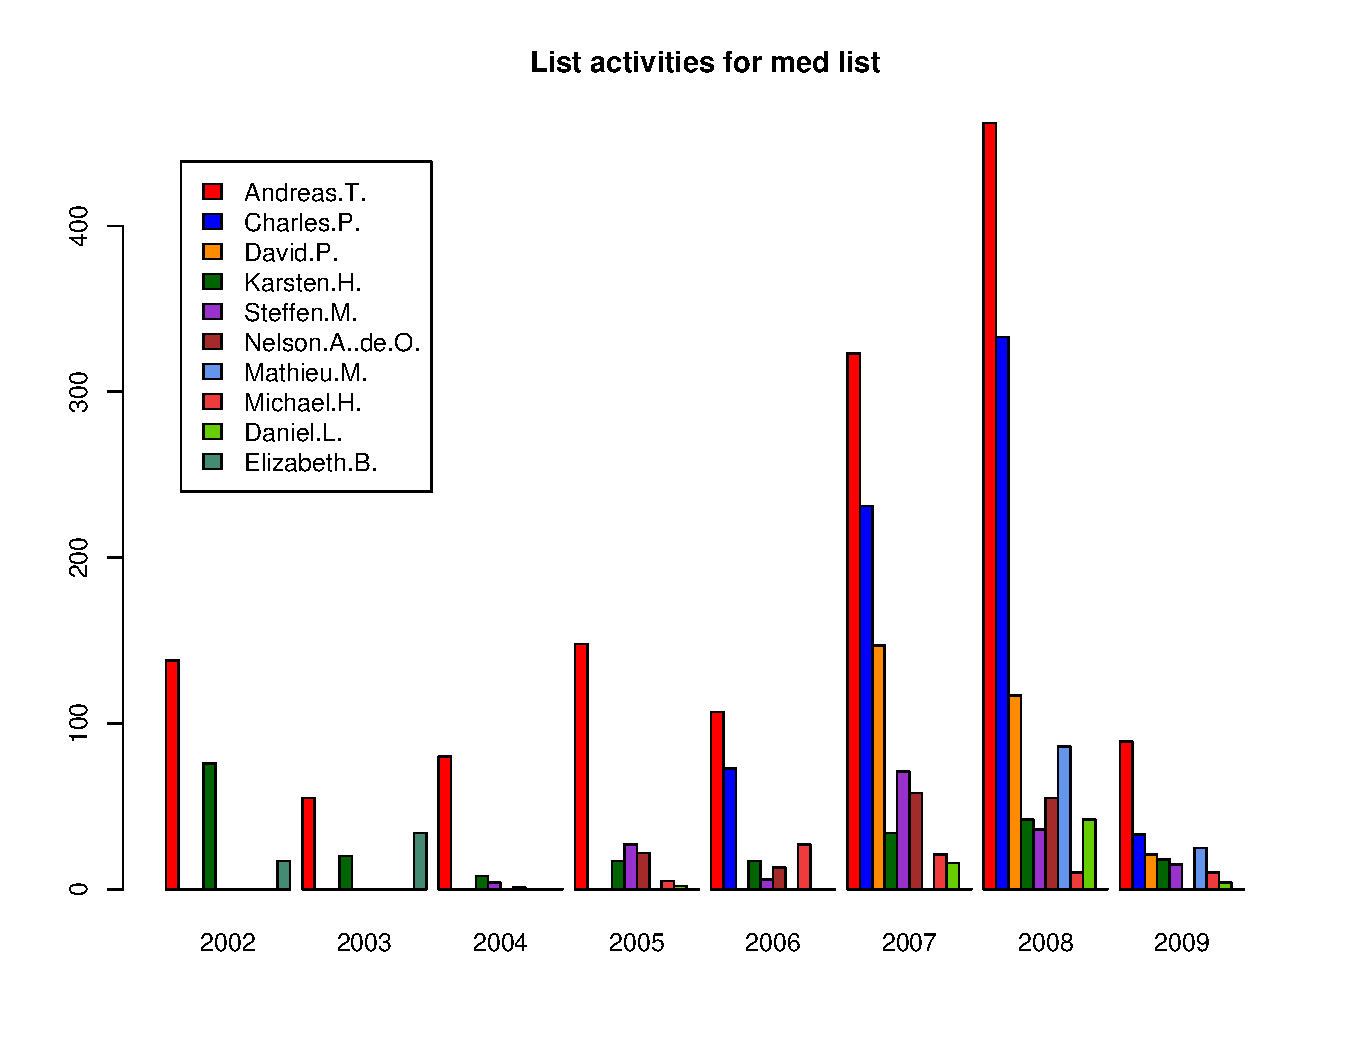
\includegraphics{authorstat_med}}
      \end{center}

\end{frame}

% Debian Edu
\begin{frame}
  \frametitle{Top 10 \link{http://lists.debian.org/debian-edu}{debian-edu@lists.debian.org}}
   \vspace{-5mm}

      \begin{center}
        \resizebox{125mm}{90mm}{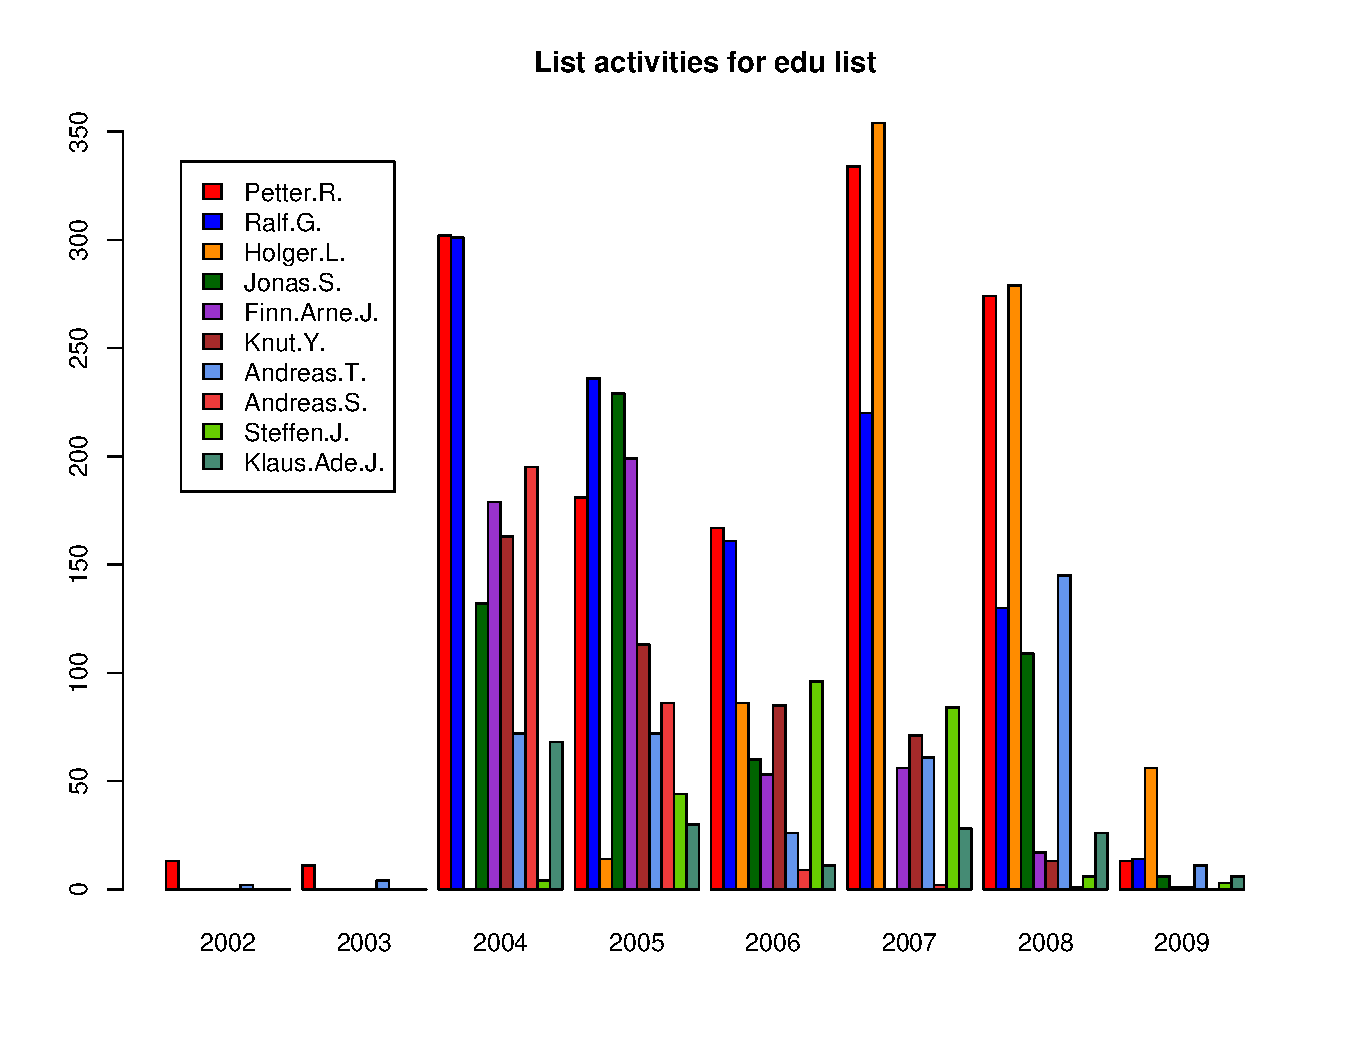
\includegraphics{authorstat_edu}}
      \end{center}

\end{frame}

% Debian Jr
\begin{frame}
  \frametitle{Top 10 \link{http://lists.debian.org/debian-jr}{debian-jr@lists.debian.org}}
   \vspace{-5mm}
        
      \begin{center}
        \resizebox{125mm}{90mm}{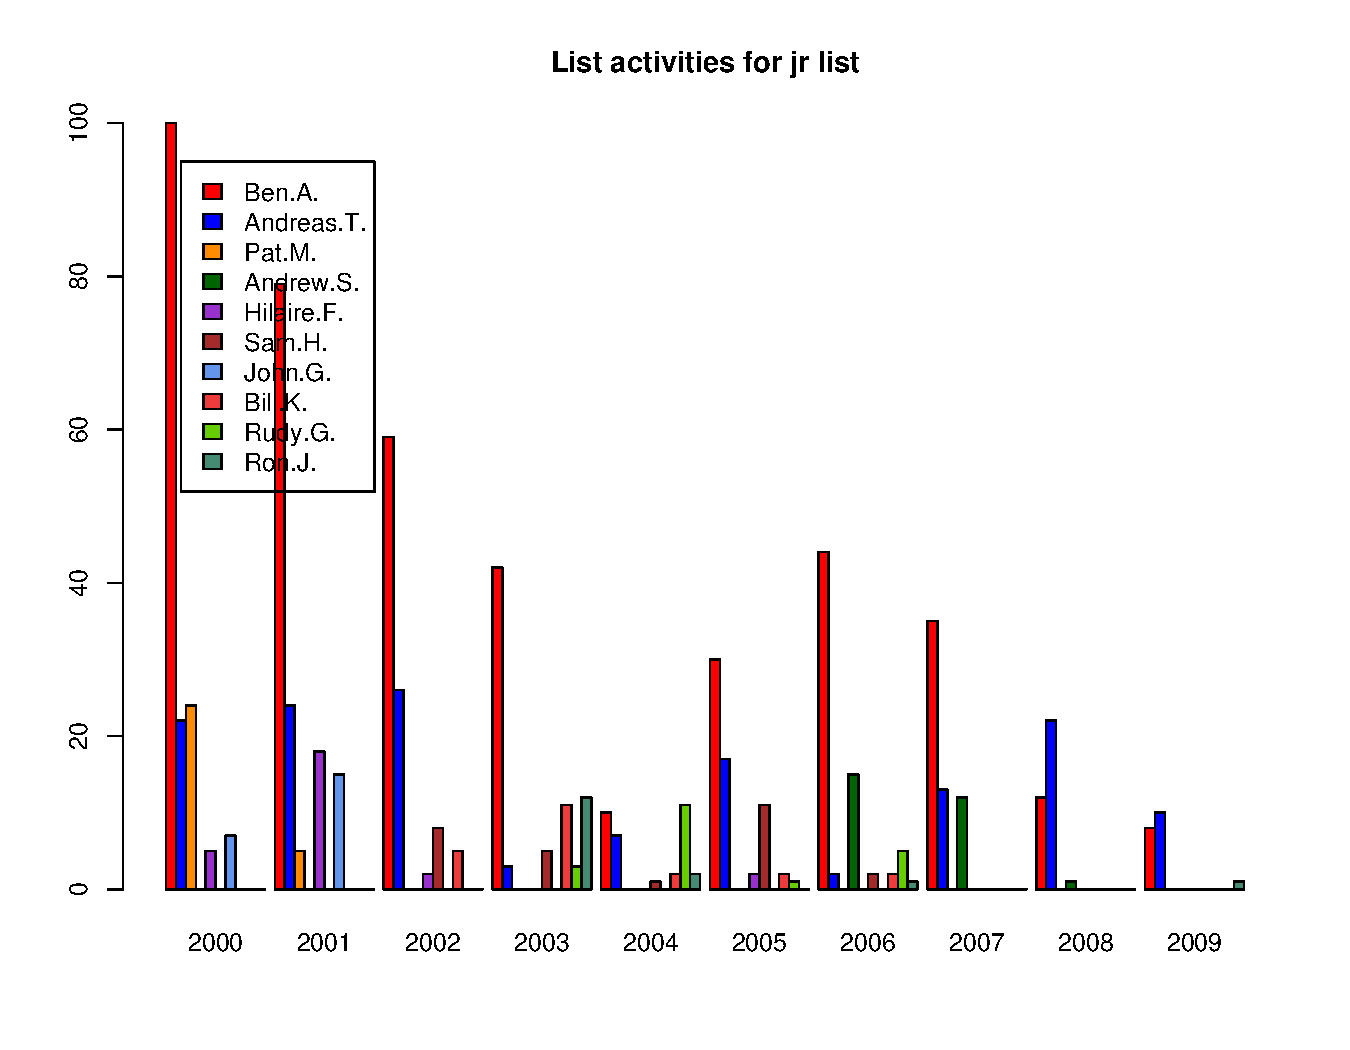
\includegraphics{authorstat_jr}}
      \end{center}
      
\end{frame}

% Debian Enterprise
\begin{frame}
  \frametitle{Top 10 \link{http://lists.debian.org/debian-enterprise}{debian-enterprise@lists.debian.org}}
   \vspace{-5mm}

      \begin{center}
        \resizebox{125mm}{90mm}{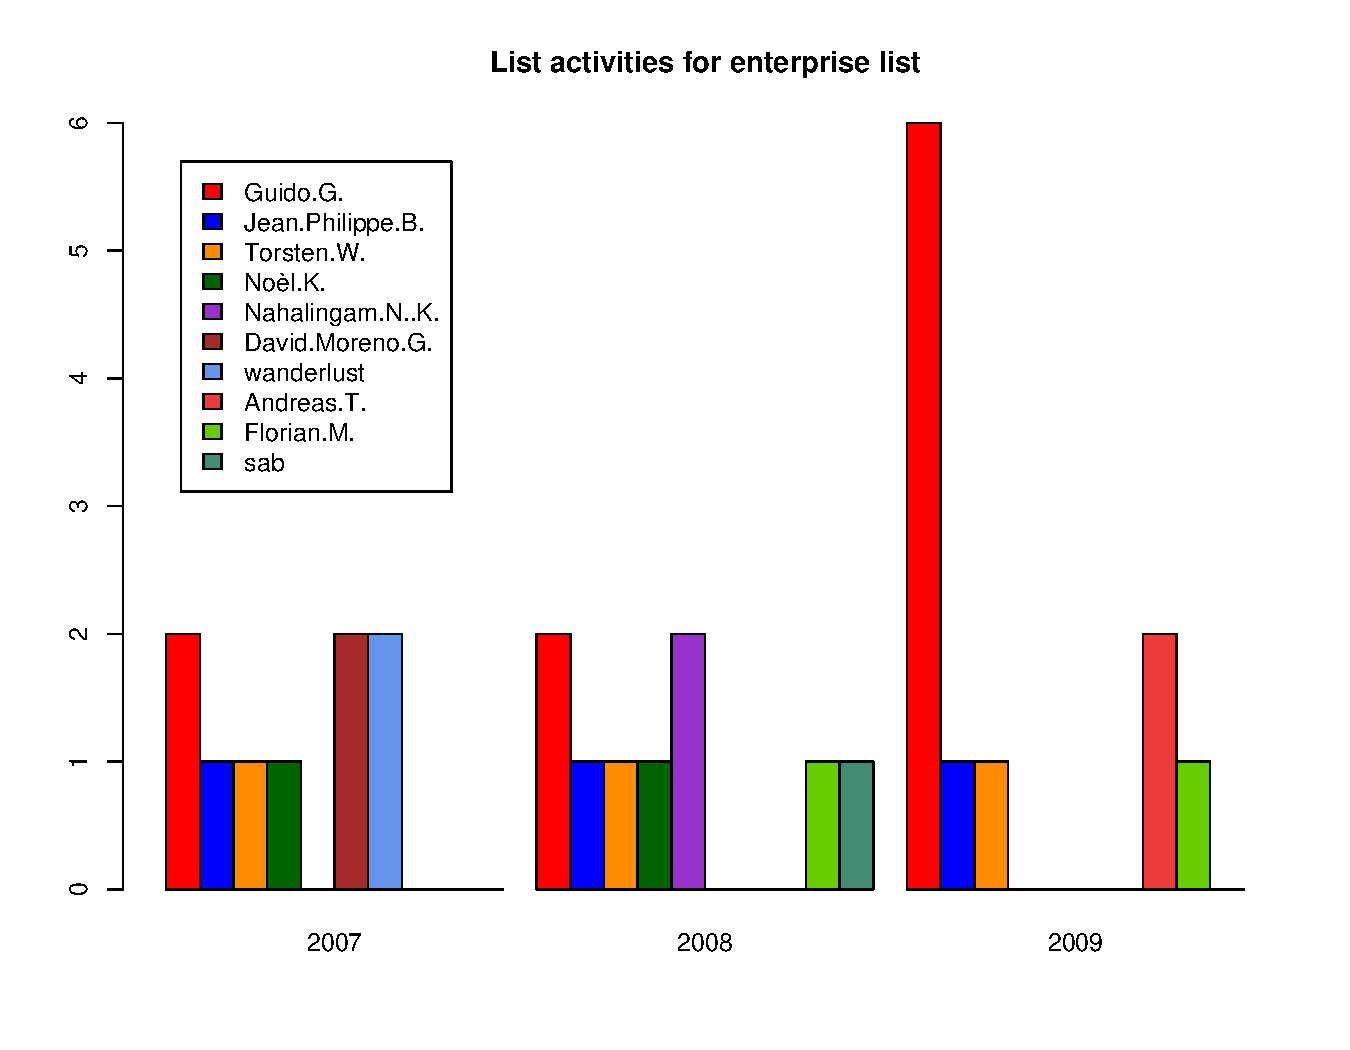
\includegraphics{authorstat_enterprise}}
      \end{center}
      
\end{frame}

%\input med-end-en.tex

\end{document}

